Синяя кривая -- фитирование лоренцовым профилем.
Черные точки -- экспериментальные данные.

\begin{figure}[h]
    \centering
    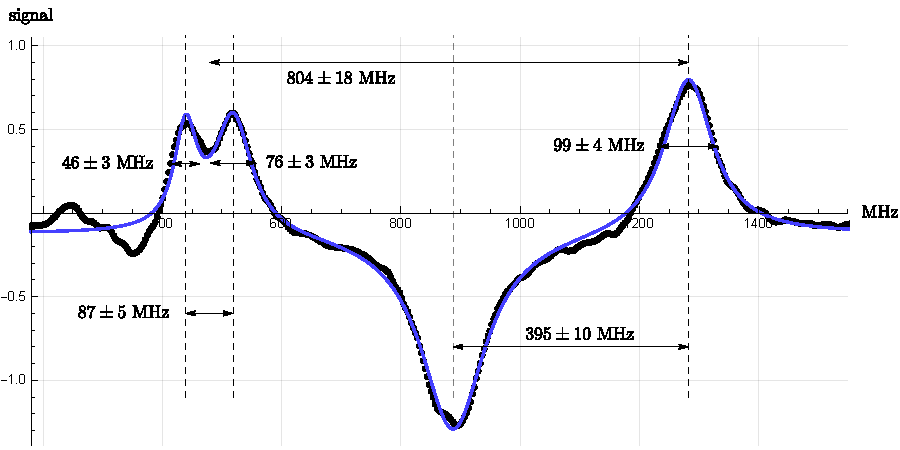
\includegraphics[width=1\textwidth]{D:\\Kami\\git_folder\\notes_5sem\\rqc\\data_processing_1\\exp_D1.pdf}
    \caption{Полученное уширение линий для D${}_1$}
    \label{fig:expD1}
\end{figure}

\vspace{-2mm}
$\Rightarrow$ Наблюдение расщепления $2 \ {}^2\text{P}_{1/2}$: $\Delta \approx 90$ МГц.